\section{Graphen}


Im allgemeinen kann ein Graph durch $G = (V, E)$ dargestellt wobei $V$ eine Menge an Knoten und $E$ eine Menge an Kanten ist. Die Kanten sind jeweils jewils ein geoordnetes Knotenpaar $(u, v) \subseteq V \times V$.

\subsection{Multi Layer Graphen}

Im folgendem werden Multi Layer Graphen betrachtet. Diese Graphen haben neben Knoten und Kanten auch eine Menge an Ebenen. Dabei kann je nach Art des Graphen der gleiche Knoten in verschiednen Ebenen vorhanden sein oder auch Verbindungen zwischen den Knoten in verschiedenen Ebenen bestehen.
Welche Bedeutung den Ebenen zukommt hängt vom Graphen und dem Anwendungsfall der Daten ab. Multi Layer Graphen können genutzt werden um Netwzerken in unterschiedlichen Themengebieten abzubilden z.B. Soziale Netwzerke, Transport oder Biologie.

Die Abbildung \ref{network_types} stellt verschiedene Arten von Multi Layer Graphen dar. 

\begin{figure}
  \centering
  \begin{subfigure}[b]{1.0\textwidth}
    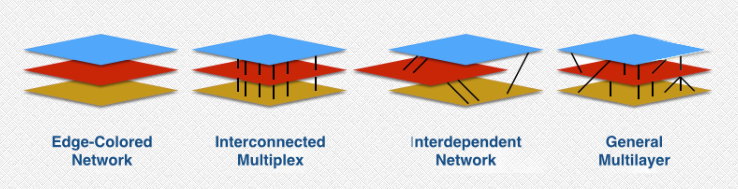
\includegraphics[width=1.0\linewidth]{img/network_types.png}
  \end{subfigure}
  \caption{Multi Layer Netzwerkarten}
  \label{network_types}
\end{figure}

\subsubsection{Edgde Colored Network}

In Edgde Colored Networks gibt es nur Kanten zwischen Knoten im gleichen Layer. Dabei sind die Kanten jeweils mit einem Label versehen zu welchem Layer sie gehören.


\subsubsection{Interconnected Multiplex}

In Multiplex Netzwerken gibt es zum einem Kanten zwischen Knotne die sich im gleichen Layer befinden. Die einzigen Kanten die es zwischen verschiedenen Layern gibt verbinden jeweils den gleichen Knoten in dem anderen Layer. 

\subsubsection{Inderdependet Network}

In Inderdependet Networks gibt es keine Knoten die in mehr als einem Layer vorkommen. Kanten können Knoten innerhalb eines Layers aber auch zwischen zwei Layern verbinden.

\subsubsection{Generelle Multi Layer}
In einem Generellen Multi Layer Graph gibt es kein Restriktion, wie die Knoten der verschiednen Ebenen miteinander verbunden sein können. Es kann sowohl Verbindungen zwischen dem gleichen Knoten in verschiedenen Ebenen geben, als auch Verbindung zu Knoten in anderen Ebenen.


Ein Genereller Mult Layer Graph kann formal als ein gerichteter Multigraph\cite{article} $G = (\Sigma_{V}, \Sigma_{E}, V, E, s, t, l_{V}, l_{E})$ dessen Knoten und Kanten ein Label besitzen  definiert werden, wo

\begin{itemize}
  \item V die Menge an Knoten und E die Menge an Kanten ist
  \item $\Sigma_{V}$ und $\Sigma{E}$ die Alphabete sind die als Label für Knoten und Kanten dienen
  \item $s: E \rightarrow V$ und $t: E \rightarrow V$ zwei Zuordnungen sind, die angeben von welchem Knoten eine Kante aussgeht und zu welchem sie führt
  \item $l_{V}: V \rightarrow \Sigma_{V}$ und $l_{E}: V \rightarrow \Sigma_{E}$ zwei Zuordnungen sind, die den Knoten und Kanten ihre Labels zuweisen
\end{itemize}

Da mit den Generellen Multilayer Graphen auch alle anderen Arten von MultiLayer Graphen dargestellt werden kann, werden im folgendem nur noch Genrelle Multigraphen betrachtet.
